\section{Nine copper coins, and other toposes}
\epigraph{
  Explicaron que una cosa es \emph{igualdad}, y otra \emph{identidad}, y formularon una especie de \emph{reductio ad absurdum}, o sea el caso hipotético de nueve hombres que en nueve sucesivas noches padecen un vivo dolor. ¿No sería ridículo -interrogaron- pretender que ese dolor es el mismo?
  }{JLB ---Tl\"on, Uqbar, Orbis Tertius}

According to our description of the Mitchell-Bénabou language in the category of variable sets, \emph{propositions} are morpisms of the form
\[p : U \to \Omega_I\]

where $\Omega_I$ is the subobject classifier of $\Set/I$ described in \ref{}; now, recall that
\begin{itemize}
  \item the object $\Omega_I = \{0,1\}\times I \to I$ becomes an object of $\Set/I$ when endowed with the projection $\pi_I : \Omega_I \to I$ on the second factor of its domain;
  \item the universal monic $\tr : I \to \Omega_I$ consists of a section of $\pi_I$, precisely the one that sends $i : I$ to the pair $(i,1) : \Omega_I$;
  \item every subobject $U \hookrightarrow A$ of an object $A$ results as a pullback (in $\Set/I$) along $\tr$:
        \[\xymatrix@R=5mm@C=5mm{
          U\ar[dr]^u\ar[rr]^u\ar[dd]_m&& I\ar[dd]^{\tr} \ar@{=}[dl]\\
          &I& \\
          A \ar[ur]\ar[rr]_{\chi_U}&& \ar[ul]\Omega_I
        }\]
        (see \ref{} for a complete proof)
\end{itemize}
The set $I$ in this context acts as a \emph{multiplier} of truth values, in that every proposition can have a pair $(\epsilon, i)$ as truth value. We introduce the following notation: a proposition $p : U \to \Omega_I$ is \emph{true}, in context $x :U$, with \emph{strength} $t$, if $p(x) =(1,t)$ (resp., $p(x)=(0,t)$).

So, a proposition is a morphism of the following kind: a function $p : U \to \Omega_I$, defined on a certain domain, and such that
\[
\xymatrix{
  U\ar[d]_u\ar[r]^-p  & \{0,1\}\times I \ar[d]^{\pi_I}\\ 
  I \ar@{=}[r]& I
}  
\]
(it must be a morphism of variable sets!) This means that $\pi p(x : U) = u(x : U)$, so that $p(x) = (\epsilon_x, u(x))$ for $\epsilon_x =0,1$ and $u$ is uniquely determined by the "variable domain" $U$. This is an important observation: the strength with which $p$ is true/false is completely determined by the structure of its domain, in the form of the function $u : U \to I$ that renders the pair $(U,u)$ an object of $\Set/I$.

To get a grip of the different roles of various classes of propositions, and given that our interest will be limited to a certain class of particular propositions that we will construct \emph{ex nihilo}, it is now convenient to discuss what constraints we have to put on the structure of $I$: of course, the richest this structure is, the better will the category $\Set/I$ behave: it is for example possible to equip $I$ with an order structure, or a natural topology. Among different choices of truth multiplier, yielding different categories of variable sets, and different kinds of internal logic therein, we will privilege those that make $I$ behave like a space of strengths: a dense, linear order with LUP, thus not really far from being a closed, bounded subset of the real line. 

The main result of the present section is a roundup of examples showing that it is possible to concoct categories of variable sets where some seemingly paradoxical constructions coming from J.L. Borges' literary world have, instead, a perfectly ``classical'' behaviour when looked with the lenses of the logic of variable set theory.

Each of the examples in our roundup \ref{bla,bli,blu,ble,blo} is organised as follows: we recall the shape of a paradoxical statement in Borges' literary world. Then, we show in which topos this reduces to an intuitive statement expressed in the syntax of a variable set category.

More than often, we use $I=[0,1]$ as base of variable sets; as already said, there are different reasons for this choice: the most intuitive is that if a truth value is given with a \emph{strength} $t\in I$ it is a natural request to be able to \emph{compare} elements in this set; in particular, it should always be possible to assess what truth value is stronger. 

For this reason, even if this assumption is never strictly necessary (the only constraint is that $I$ is totally, or partially, ordered set by a relation $\le$), a natural choice for $I$ is a \emph{continuum} (=a dense total order with LUP --see \cite{descriptive-set-theory}). An alternative choice drops the density assumption: in that case the (unique) finite total order $\Delta[n] = \{0 < 1 <\dots < n\}$, or the countable total order $I=\omega = \bigcup_n \Delta[n]$ are all pretty natural choices for $I$ (although it is way more natural for $I$ to have a minimum \emph{and} a maximum element).\footnote{We're oly interested in the notion of an abstract interval here: a continuum $X$ endowed with an operation $X \to X \vee X$ of ``zooming'', uniquely defined by this property. In a famous paper Freyd characterises ``the interval'' as the terminal interval coalgebra: see \cite[]{}; for our purposes, note that $[0,1]$ is a natural choice: it is a frame, thus a Heyting algebra $\fkH =([0,1],\land,\lor,\Rightarrow)$ with respect to the pseudo-complement operation given by $(x \Rightarrow z) := \bigvee_{x\land y \le z} y$ (it is immediate that $x \land a \le b$ if and only if $a \le x \Rightarrow b$ for every $a,b\in [0,1]$).} In each of these cases ``classical'' logic is recovered as a projection: propositions $p$ can be true or false with strength $1$,\footnote{Here $I$ is represented as an interval whose minimal and maximal element are respectively $0$ and $1$; of course these are just placeholders, but it is harmless for the reader to visualise $I$ as the interval $[0,1]$.} the maximum element of $I$:
\begin{center}
  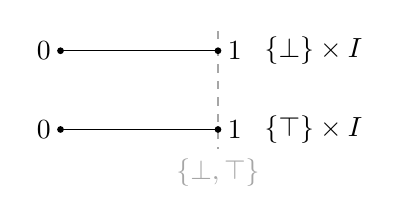
\begin{tikzpicture}
    \draw[gray!70,dashed] (2,1.25) -- (2,-.25) node[below] {$\{\perp,\top\}$};
    \draw[fill] (0,0) circle (1pt) node[left] {$0$};
    \draw[fill] (2,0) circle (1pt) node[right] (dis) {$1$};
    \draw (0,0) -- (2,0);
    \begin{scope}[yshift=1cm]
    \draw[fill] (0,0) circle (1pt) node[left] {$0$};
    \draw[fill] (2,0) circle (1pt) node[right] (dat) {$1$};
    \draw (0,0) -- (2,0);
    \node[right of=dis] {$\{\top\}\times I$};
    \node[right of=dat] {$\{\perp\}\times I$};
    \end{scope}
    \end{tikzpicture}
\end{center}
In order to aid the reader understand the explicit way in which $I$ ``multiplies'' truth values, we spell out explicitly the structure of the subobject classifier in $\Set/\Delta[2]$. In order to keep calling the minimum and maximum of $I$ respectively $0$ and $1$ we call $\frac{1}{2}$ the intermediate point of $\Delta[2]$.
\begin{remark}
The subobject classifier of $\Set/\Delta[2]$ consists of the partially ordered set $\Delta[1]\times\Delta[2]$ that we can represent pictorially as a rectangle
  \[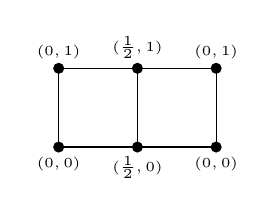
\begin{tikzpicture}[xscale=2]
    \foreach \i/\name in {0/0,.5/{\frac{1}{2}},1/0}{
      \foreach \j/\pos in {0/below,1/above}
        \fill (\i,\j) ellipse (1pt and 2pt) node[\pos] {\tiny $(\name,\j)$};
    }
    \draw (0,0) rectangle (1,1);
    \draw (.5,1) -- (.5,0);
    \end{tikzpicture}\]
  endowed with the product order. The resulting poset is partially ordered, and in fact a Heyting algebra, because it results as the product of two Heyting algebras: the Boole algebra $\{0<1\}$ and the frame of open subsets of the Sierpinski space $\{a,b\}$ (the topology is $\tau_S = \{\varnothing, \{a\}, \{a,b\}\}$).
  \end{remark}
  \begin{remark}
    Siccome il caso $I=[0,1]$ con la topologia euclidea è quello piu naturale per diversi motivi, definiamo alcuni insiemi di interesse per una data proposizione $p : U \to \Omega_I$ per questa scelta di $I$:
  \begin{itemize}
    \item $A^\top = \{x : U \mid p(x) = (1,t_x), t_x > 0\} = p^\leftarrow(\{1\}\times (0,1])$ e $A^\perp = \{x : U \mid p(x) = (0,t_x), t_x > 0\}$; cose vere (risp., false) con forza maggiore di zero. Sono le funzioni $u : U \to I$ tali che $u^\leftarrow 0 = \varnothing$.
    \item $B^\top = \{x : U \mid p(x) = (1,1)\} = p^\leftarrow((1,1))$ e $B^\perp = \{x : U \mid p(x) = (0,1)\}$ cose vere (risp.,false).
    \item $E_t^\top = \{ x : U \mid p(x)=(1,t)\}$ e $E_t^\perp = \{ x : U \mid p(x)=(0,t)\}$; cose vere (risp., false) con forza $t$.
  \end{itemize}
  \end{remark}
  Last but not least, a crucial assumption will be that the strength of $p$ depends continuously, or not, on the variables on its domain of definition. Without such continuous dependence, small changes in context $x : U$ might drastically change the truth value $p(x)$.\footnote{There is no a priori reason to maintain that $p$ is a continuous proposition; one might argue that discontinuous changes in truth value of $p$ happen all the time in ``real life''; see the family of paradoxes based on so-called \emph{separating instants}: how well-defined the notion of ``time of death'' is? How well-defined the notion of ``instant in time''?}
\subsection{The unimaginable topos theory hidden in Borges' library}
L'opera letteraria di Borges è famosa per avere creato universi paradossali, retti da leggi controintuitive ma allo stesso tempo inescapabilmente coerenti; tra i temi costanti di riflessione nei suoi scritti spunta una matematica molto raffinata, e riflessioni profonde sull'infinito, la duplicazione, l'autoreferenzialità, la ricorsione, la periodicità, la natura illusoria del tempo, i paradossi della logica, i limiti del linguaggio e, ovviamente, le ricadute di ciascuno di questi argomenti sulle nostre stance ontologiche.

E' quindi naturale sceglierlo sia come rappresentante illustre del nostro modo di operare, e delle suggestioni che lo hanno ispirato, sia come factory of examples di logiche 

A voler trovare un risultato originale in questo scritto, esso sta proprio nell'avere sottolineato come i mondi alternativi di Borges (Babilonia, Tl\"on\dots) sono matematicamente fondati. E lo sono esattamente grazie a una teoria dell'esistenza base-relative, dove non esiste un'unica ontologia, ma invece ne esiste una per ogni universo che si va costruendo.
\begin{example}[Nine copper coins]
  la freccia, le monete. Rammentiamo il paradosso da \cite{}:\footnote{The translation we employ is classical and comes from \cite{}: 
  \begin{quote}
    \hspace{.5em} Tuesday, X crosses a deserted road and loses nine copper coins. On Thursday, Y finds in the road four coins, somewhat rusted by Wednesday's rain. On Friday, Z discovers three coins in the road. On Friday morning, X finds two coins in the corridor of his house. The heresiarch would deduce from this story the reality - i.e., the continuity - of the nine coins which were recovered. 
    
    \hspace{.5em} It is absurd (he affirmed) to imagine that four of the coins have not existed between Tuesday and Thursday, three between Tuesday and Friday afternoon, two between Tuesday and Friday morning. It is logical to think that they have existed - at least in some secret way, hidden from the comprehension of men - at every moment of those three periods. 
  \end{quote}}
  \begin{quote}
    El martes, $X$ atraviesa un camino desierto y pierde nueve monedas de cobre.
    El jueves, $Y$ encuentra en el camino cuatro monedas, algo herrumbradas por la lluvia del miércoles. El viernes, $Z$ descubre tres monedas en el camino. El viernes de mañana, $X$ encuentra dos monedas en el corredor de su casa. El  quería deducir de esa historia la realidad -id est la continuidad- de las nueve monedas recuperadas. 
    
    Es absurdo (afirmaba) imaginar que  cuatro de las monedas no han existido entre el martes y el jueves, tres entre el martes y la tarde del viernes, dos entre el martes y la madrugada del viernes. Es lógico pensar que han existido -siquiera de algún modo secreto, de comprensión vedada a los hombres- en todos los momentos de esos tres plazos.
  \end{quote}
  Before going on with our analysis, two remarks are in order:
  \begin{itemize}
    \item the paradox appears in a primitive version in \cite{}, where instead of nine copper coins, a single arrow, shot by an anonymous archer, disappears among the woods. The text appears in a hard-to-find edition of \emph{Inquisiciones} (\cite{}); in the last chapter, we read the \emph{avatar de la flecha}:
\begin{quote}
    X scocca una freccia da un arco, ed essa si perde fra gli alberi.
    
    X la cerca e riesce a ritrovarla.
    
    E' assurdo immaginare che la freccia non sia esistita durante il periodo fra i momenti in cui X l'ha persa di vista e l'ha ritrovata.
    
    E' logico pensare che essa sia esistita - anche se in un certo modo segreto, di comprensione vietata agli uomini - in tutti i momenti di questo periodo.
\end{quote}
    \item There is one and only one reason why the paradox of the nine copper coins is invalid: copper does not rust.
  \end{itemize}
  Nel seguito, ci concentriamo sul paradosso come enunciato nella sua forma più recente; ignoriamo quindi la formulazione precedente, data in termini di una freccia. Non solo: offriamo una rettificazione alla ``critica della ruggine'', che non si basa sull'ipotesi (vietata in una prospettiva di igiene occamista) che oltre alla metafisica, anche la fisica di Tl\"on abbia comportamenti diversi da quelli sulla terra.

  In linguaggio naturale, le cose vanno circa come segue: $X$ perde le monete, e la forza con cui esse ``esistono'' si abbassa; cresce, e torna massima, ma non per tutte le monete, quando X le ritrova sul portone,  e $Y$ ne trova altre arrugginite per la pioggia (ma siccome il rame non arrugginisce, non sono arrugginite "a causa" della pioggia: in una sorta di principio di wormhole, eventi indipendenti sulla terra sono dipendenti su Tlön, perché l'evento A influenza, in uno spazio pluridimensionale di scelte di z di verità, l'evento B in modi che gli sarebbero vietati se fosse sulla Terra.) $\Omega_I = \{0<1\}\times I$ dove $I$ è un qualsiasi insieme con più di un elemento; esempio minimale, $I=\{N,S\}$ (suddivisione del mondo, e delle ontologie del mondo, in due emisferi), esempio psicologicamente interessante: $I=[0,1]$ (c'è un continuo non numerabile di forze distinte con cui una proprietà può essere vera o falsa); $[0,1]$ è anche il luogo standard dove interpretare logiche sfumate, sebbene lì in senso probabilistico.

  Ora, per formalizzare la situazione procediamo come segue: senza perdita di generalità possiamo supporre l'insieme $C = \{c_1,\dots,c_9\}$ delle monete totalmente ordinato e partizionato in modo tale che le prime due monete siano quelle ritrovate da $X$ il martedì, le seconde quattro quelle che $Y$ ritrova sul cammino, e le ultime 3 quelle viste da $Z$. Allora
  \[C = C_X \sqcup C_Y \sqcup C_Z.\]
  L'insieme $I$ è l'intervallo $[0,1]$; non operiamo l'identificazione $(\top,0) \sim (\perp,1)$ o $(\perp,0) = (\top,1)$.

  Le proposizioni di cui ci occupiamo sono della forma
  \[\lambda gcd.p(g, c, d) : \{X,Y,Z\}\times C\times W \to \Omega_I\]
  dove $W$ è l'insieme dei giorni della settimana, e $d : W$ assume valori $L,M,M,\dots,D$ (sebbene nel paradosso intervenga il sottoinsieme $W'$ dei soli giorni $[Ma,Ve]$).

  Definiamo ora \emph{ammissibile} una configurazione tale che le condizioni seguenti sono rispettate: 
  \[
  \begin{cases}
    \prod_{c:C, d:W} \sum_{u\in \{X,Y,Z\}} p(u,c,d) = (\top, 1) \\ 
    p(X,c_X,V) = (\top,1)\\
    p(Y,c_Y,G) = (\top,1)\\
    p(Z,c_Z,V) = (\top,1)
  \end{cases}  
  \]
  In ogni configurazione ammissibile l'esistenza \emph{parziale} delle monete, ossia l'esistenza dei sottoinsiemi $C_X,C_Y,C_Z$ può essere minore del massimo; per un osservatore esterno capace di sommare le forze con cui le varie parti di $C$ esistono, tuttavia, le monete esistono ``in qualche modo segreto, di comprensione vietata agli uomini'' (or rather, to $X,Y,Z$).
\end{example}
\begin{example}
  la lotteria a Babilonia: proposizioni $p : U \to \Omega_{[0,1]}$ possono essere fortemente discontinue: allora esse descrivono un evento innescato come termine finale di una catena di eventi apparentemente disconnessi e paradossali;\footnote{Assumendo una base reale per lo spazio dei parametri da cui $p$ dipende, la sua dipendenza continua è la seguente proprietà: \dots; ciò significa che eventi vicini --nello spazio o nella consequenzialità-- non possono avere valori di verità diversi} in questo mondo, un modello del quale è probabilmente la Babilonia dei ``sorteggi impersonali, di proposito indefinito'', azioni apparentemente scorrelate tra loro (scagliare ``nelle acque dell'Eufrate uno zaffiro di Taprobana''; sciogliere ``dal tetto d'una torre [\dots\unkern] un uccello''; togliere (o aggiungere) ``un granello di rena ai grani innumerevoli della spiaggia'', hanno ``conseguenze, a volte, tremende''.
\end{example}
\begin{example}
  Per quanto riguarda le proposizioni che sono continue nelle proprie variabili, invece, esempio canonico sono le ``tigri di cristallo'' e le ``torri di sangue'' di Tl\"{o}n: oggetti ed entità usuali, diversi da quelli ``classici'' per un dettaglio solo (il colore, la consistenza, il materiale di cui sono composte). Oppure dipendenti in maniera \emph{monotona} e continua dai loro paramentri: $p$ è tanto più vera quanta più gente la osserva, perché ``Le cose, su Tlön, si duplicano; ma tendono anche a cancellarsi e a  perdere i dettagli quando la gente le dimentichi. È classico l'esempio di  un'antica soglia, che perdurò finchè un mendicante venne a visitarla, e che alla  morte di colui fu perduta di vista. Talvolta pochi uccelli, un cavallo, salvarono le  rovine di un anfiteatro. ''
        \[\textstyle p(\exists\text{rovine dell'anfiteatro}, n) = \big(\top, 1-\frac{1}{n}\big)\]
        se $n$ è il numero di persone che vede l'anfiteatro.
\end{example}
\begin{example}
  Il Berkeley idealista degli infiniti istanti di tempo continuo, disconnessi e incomunicabili: $\Omega_I = \coprod_{t : [0,1]} \{ 0 < 1 \}$. E' evidente come questa struttura logica influenzi il linguaggio: i termini sono costruiti per accrezione istantanea, per somma disgiunta dei costituenti e delle loro proprietà: ``aereo-chiaro sopra scuro rotondo''; oggetti determinati dalla sola simultaneità, più che da una dipendenza logica. Altra conferma di ciò, l'abbandono della consequenzialità temporale sta nel passo ``Spinoza attribuisce alla sua inesauribile divinità i modi del pensiero e dell'estensione; su Tlön, nessuno comprenderebbe la giustapposizione del  secondo (che caratterizza solo alcuni stati) e del primo, che è un sinonimo  perfetto del cosmo. In altre parole: non concepiscono che lo spaziale perduri  nel tempo. La percezione di una fumata all'orizzonte, e poi della campagna  incendiata, e poi della sigaretta mal spenta che provocò l'incendio, è  considerata un esempio di associazione di idee.'' Ciò si lega anche al passo ``L'universo è paragonabile a quelle crittografie in cui non tutti i segni hanno un valore, e che solo è vero ciò che accade ogni trecento notti'': un mondo dove ogni trecento notti $p(x) =(\top,1)$, e per le successive 299 notti $p$ ha forza $<1$.
\end{example}
\begin{example}
  
\end{example}
